% advsph.tex

\chapter{\'Equation d'advection sphérique}

Nous présentons dans cette parties les tests et les résultats numériques associés pour l'équation d'advection :
\begin{equation}
\label{eq:advection spherique}
\left\lbrace
\begin{array}{r cl}
\dfrac{\partial h}{\partial t} + \mathbf{c} ( \mathbf{x} ) \cdot \nabla_ T h & = & 0 \\
h(\mathbf{x},0) & = & h_0 ( \mathbf{x} )
\end{array}
\right. \text{ pour tout } \mathbf{x} \in \mathbf{S}_a^2 \text{ et } t \geq 0
\end{equation}

La solution exacte est donnée pour tout ces tests, on peut mesurer l'erreur relative au temps $t^n$ avec :

\begin{equation}
\label{erreur relative}
e(t^n) = \dfrac{\| h^n - h(t^n) \|_p}{\| h(t^n) \|_p}
\end{equation}

où $h^n$ est la solution numérique au temps $t^n$ et $h(t^n)$ la solution exacte au même instant. $p \in {1, 2, \infty }$ permet de choisir la norme de notre choix.

Dans la suite, nous adoptons le schéma en temps Runge-Kutta d'ordre 4 détaillé précédemment. La discrétisation en espace se fait via les schéma hermitiens construits sur la Cubed-Sphere utilisant les schémas compacts d'ordre 4. On notera à présent la condition de Courant-Friedrich-Lewis (notée CFL) :

\begin{equation}
CFL = \dfrac{u_0 \times \Delta t}{a \times \Delta \xi} = \dfrac{u_0 \times \Delta t}{a \times \Delta \eta}
\end{equation}

\section{Préliminaires}

Soit $\mathbf{x} = (x,y,z)^T \in \mathbb{S}_a^2$ un point de la sphère de centre $O$ et de rayon $a$. Il existe alors $\lambda$ et $\theta$ , respectivement longitude et latitude, dans $] 0, 2 \pi ] \times ] - \pi /2, \pi/2 [ $ tels que :

\begin{equation}
\left\lbrace 
\begin{array}{rcl}
x & = & a \cos \theta \cos \lambda \\
y & = & a \cos \theta \sin \lambda \\
z & = & a \sin \theta
\end{array}
\right.
\end{equation}

Si le point $\mathbf{x}$ se déplace le long de la sphère $\mathbb{S}^2_a$, le vecteur vitesse de ce point est donnée par la formule :

\begin{equation}
\dfrac{d \mathbf{x}}{dt} = u \mathbf{e}_{\lambda} + v \mathbf{e}_{\theta}
\end{equation}

où $\mathbf{e}_{\lambda}$ et $\mathbf{e}_{\theta}$ sont donnés en annexe dans la remarque \ref{base_lonlat}. 

Par identification, on a :

\begin{equation}
\left\lbrace 
\begin{array}{rcl}
u & = & a cos ( \theta ) \dfrac{d \lambda}{dt} \\
v & = & a \dfrac{d \theta}{dt}
\end{array}
\right.
\end{equation}

Lorsque $\mathbf{x}$ est transporté parallèlement à l'équateur, à vitesse angulaire constante, seul sa latitude varie. On a donc :

\begin{equation}
\left\lbrace 
\begin{array}{rcl}
\dfrac{d \lambda}{dt} & = & \omega \\
\dfrac{d \theta}{dt} & = & 0
\end{array}
\right.
\end{equation}

Supposont à présent que $P=( \lambda_P, \theta_P)$ est un point de $\mathbb{S}_a^2$. Un nouveau système de coordonnées est donné en placant le nouveau pôle Nord en $P$ au lieu du pôle Nord habituel. Dans ce système, les points sont positionnés en $(\lambda', \theta')$ (en longitude-latitude "tournée") et en $(\lambda, \theta)$ dans le système de coordonnés classiques (en longitude-latitude).

Pour des raisons pratiques, nous avons besoin des relations permettant de passer de $( \lambda', \theta')$ à $(\lambda, \theta)$ et inversement.

En utilisant les relations de trigonométrie sphèrique, on a :

\begin{equation}
\label{coord_rot}
\left\lbrace 
\begin{array}{rcl}
sin ( \theta ) & = & sin( \theta_P) sin( \theta') - cos( \theta_P) cos( \theta') cos( \lambda' ) \\
sin( \theta' ) & = & sin( \theta) sin(\theta_P) + cos( \theta ) cos( \theta_P) cos( \lambda - \lambda_P ) \\
cos( \theta ) sin( \lambda - \lambda_P) & = & cos( \theta' ) sin( \lambda' )
\end{array}
\right.
\end{equation}.

En utilisant (\ref{coord_rot}.b), la formule suivante est immédiate :

\begin{equation}
\theta' = arcsin \left[ sin( \theta) sin(\theta_P) + cos( \theta ) cos( \theta_P) cos( \lambda - \lambda_P ) \right]
\end{equation}

De plus, (\ref{coord_rot}.a) et (\ref{coord_rot}.c) donnent :

\begin{equation}
\left\lbrace 
\begin{array}{rcl}
cos( \theta ) sin( \lambda - \lambda_P) & = & cos( \theta' ) sin( \lambda' ) \\
cos( \theta ) cos( \lambda - \lambda_P) & = & \frac{sin( \theta' ) sin ( \theta_P ) - sin( \theta )}{cos( \theta_P)}
\end{array}
\right.
\end{equation}.

Or :

\begin{equation*}
\begin{array}{rcl}
cos( \theta ) cos( \lambda - \lambda_P) & = & \dfrac{sin( \theta' ) sin ( \theta_P ) - sin( \theta )}{cos( \theta_P)} \\
 & = & \dfrac{sin( \theta) (sin^2 ( \theta_P) -1 )}{cos( \theta_P)} + cos( \theta ) cos( \lambda- \lambda_P) sin( \theta_P)\\
 & = & cos ( \theta) cos( \lambda - \lambda_P) sin( \theta_P ) - sin( \theta) cos ( \theta_P )
\end{array}
\end{equation*}

Dès lors, en remarquant que :

$$tan ( \lambda' ) =  \dfrac{cos( \theta' ) sin(  \lambda' ) }{cos( \theta' ) cos(  \lambda' )}$$

on a le changement de coordonnées dans un premier sens :

\begin{equation}
\label{from classic to prime}
\left\lbrace 
\begin{array}{rcl}
\theta' & = & arcsin \left[ sin( \theta) sin(\theta_P) + cos( \theta ) cos( \theta_P) cos( \lambda - \lambda_P ) \right] \\
\lambda' & = & arctan \left[ \dfrac{cos ( \theta) sin( \lambda - \lambda_P)}{cos( \theta) cos( \lambda - \lambda_P) sin( \theta_P) - sin( \theta) cos( \theta_P)} \right]
\end{array}
\right.
\end{equation}

Inversement et par une démonstration similaire, on a :

\begin{equation}
\label{from prime to classic}
\left\lbrace 
\begin{array}{rcl}
\theta & = & arcsin \left[ sin( \theta') sin(\theta_P) - cos( \theta' ) cos( \theta_P) cos( \lambda' ) \right] \\
\lambda & = & \lambda_P + arctan \left[ \dfrac{cos ( \theta') sin( \lambda ')}{sin( \theta') cos( \theta_P) + cos ( \theta') cos( \lambda') sin ( \theta_P)} \right]
\end{array}
\right.
\end{equation}

Si le point $\mathbf{x}$ est transporté parallèlement au nouvel équateur, on a :

\begin{equation}
\left\lbrace 
\begin{array}{rcl}
\dfrac{d \lambda'}{dt} & = & \omega \\
\dfrac{d \theta'}{dt} & = & 0
\end{array}
\right.
\end{equation}.

où $\omega$ est la vitesse angulaire.

En dérivant (\ref{coord_rot}.a) par rapport à $t$, on a :

\begin{equation}
\begin{array}{rcl}
\dfrac{d \theta}{dt} cos ( \theta ) & = & \dfrac{d \lambda' }{dt} cos ( \theta' ) cos ( \theta_P) sin( \lambda') \\
 & = & \omega cos ( \theta' ) cos ( \theta_P) sin( \lambda') \\
 & = & \omega cos ( \theta ) cos ( \theta_P) sin( \lambda) \text{ par (\ref{coord_rot}.c)}\\
\end{array}
\end{equation}

d'où par identification :

\begin{equation}
\label{vitesse_solide_v}
v = a \omega cos ( \theta_P ) sin( \lambda - \lambda_P )
\end{equation}

De la même manière, avec \ref{coord_rot}.b), on a :

\begin{equation}
\label{vitesse_solide_u}
u = a  \omega \left( cos ( \theta ) sin( \theta_P) - sin( \theta ) cos( \theta_P) cos( \lambda - \lambda_P) \right)
\end{equation}

\section{Test de rotation solide}

L'idée dans cette partie est de présenter un test pour l'équation d'advection \eqref{eq:advection spherique} transportant la condition initiale le long d'un grand cercle.

\subsection{Cas 1 : transport parallère à l'équateur}

Le but de cette partie est de résoudre l'équation d'advection sphèrique suivante :

\begin{equation}
\label{eq:advection spherique 1}
\left\lbrace
\begin{array}{r cl}
\dfrac{\partial h}{\partial t} + \mathbf{c} ( \mathbf{x} ) \cdot \nabla_ T h & = & 0 \\
h(\mathbf{x},0) & = & h_0 ( \mathbf{x} )
\end{array}
\right. \text{ pour tout } \mathbf{x} \in \mathbf{S}_a^2 \text{ et } t \geq 0
\end{equation}

Avec $\mathbf{c} ( \mathbf{x} ) = a \omega cos ( \theta ) \mathbf{e}_{\lambda}$ le vecteur de transport \footnote{Dans ce premier cas, le transport est parallèle à l'équateur et à vitesse constante.}.
On cherche la solution par la méthode des caractéristiques, sur la caractéristique $t \rightarrow\mathbf{x}(t) = (\lambda (t), \theta(t) )$ on a :

\begin{equation}
\left\lbrace
\begin{array}{rcl}
\partial_t \lambda & = & u_0 cos ( \theta ) \\
\partial_t \theta & = & 0
\end{array}
\right.
\end{equation}

d'où : $\lambda(t) = \lambda_0 + \Omega t$ et $\theta(t) = \theta_0$ avec $\Omega = u_0 cos ( \theta )$.

Ainsi la solution de \eqref{eq:advection spherique 1} est :

\begin{equation}
\label{eq: advection solution 1}
h( \mathbf{x}, t ) = h_0 ( \lambda - \Omega t, \theta ) = h_0 ( R_{-t}  \mathbf{x} )
\end{equation}

Avec $R_{-t}$ la rotation autour de l'axe $(Oz)$ d'angle $-\Omega t$ autour de l'axe :

\begin{equation}
\label{rotation}
R_{-t} = \begin{pmatrix}
cos \left( - \Omega t \right) & -sin \left( - \Omega t \right) & 0\\
sin \left( - \Omega t \right) & cos \left( - \Omega t \right)  & 0\\
0 & 0 & 1 \\
\end{pmatrix}
\end{equation}

\subsection{Cas 2 : transport parallèle à un grand cercle}

On souhaite résoudre l'équation \eqref{eq:advection spherique 1} avec $\mathbf{c}$ donné en chaque point par :

$$\mathbf{c} ( \mathbf{x} ) = u_0 ( cos ( \theta) cos ( \alpha ) + sin( \theta) cos ( \lambda) sin( \alpha) ) \mathbf{e}_{\lambda} - u_0 sin( \lambda) sin( \alpha) \mathbf{e}_{\theta}. $$

On reconnait la forme donnée par \eqref{vitesse_solide_v} et \eqref{vitesse_solide_u} lorsque $u_0 = a \omega$ ainsi que $(\lambda_P, \theta_P) = (\pi, \pi/2 - \alpha)$ (Voir figure \ref{fig:rot alpha sphere}). 

\begin{figure}[ht]
\begin{center}
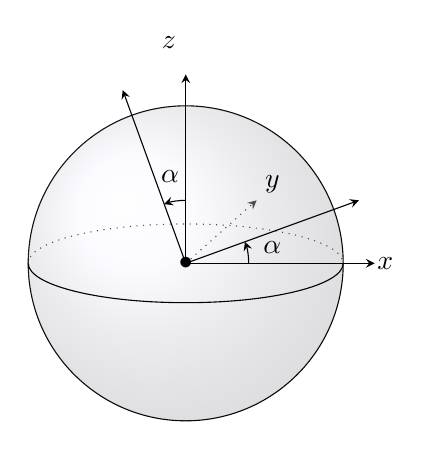
\begin{tikzpicture}[scale=2]
\draw (0,0) circle (1) ;
\shade[ball color=blue!10!white,opacity=0.20] (0,0) circle (1);
\draw (-1,0) arc (180:360:1cm and 0.25cm);
\draw (-1,0)[dotted, color=black!70] arc (180:360:1cm and -0.25cm);

\draw [>=stealth, ->] (0,0) -- (1.1,0.4) ;
\draw [>=stealth, ->](0.4,0) arc (0:20:0.4cm);
\draw (0.55,0.1) node{$\alpha$} ; 
\draw [>=stealth, ->] (0,0) -- (-0.4,1.1) ;
\draw [>=stealth, ->](0,0.4) arc (90:110:0.4cm);
\draw (-0.1,0.55) node{$\alpha$} ; 

\draw [>=stealth, ->] (0,0) -- (1.2,0) ;
\draw (1.38,0) node[left]{$x$} ;   
\draw [>=stealth, ->] (0,0) -- (0,1.2) ;
\draw (0,1.4) node[left]{$z$} ;  

\draw [>=stealth, ->, dotted, color=black!70] (0,0) -- (0.45,0.4) ;
\draw (0.55,0.5) node{$y$} ; 
\draw (0,0) node {$\bullet$} ; 

\end{tikzpicture}
\end{center}
\caption{Axes $(NS)$ tourné d'un angle $\alpha$.}
\label{fig:rot alpha sphere}
\end{figure}





Le gradient $\nabla_T h$ est invariant par rotation, on peut donc effectuer le changement de variable $\mathbf{x}' = P_{\alpha}^{-1} \mathbf{x}$ dans \eqref{eq:advection spherique 1}. $P_{\alpha}$ est la rotation autour de $(Oy)$ d'angle $\alpha$.

On obtient alors :

\begin{equation}
\left\lbrace
\begin{array}{r cl}
\dfrac{\partial h}{\partial t}( \mathbf{x}' ) + \mathbf{c} ( \mathbf{x}' ) \cdot \nabla_ T h( \mathbf{x}' ) & = & 0 \\
h(\mathbf{x}',0) & = & h_0 ( \mathbf{x}' )
\end{array}
\right. \text{ pour tout } \mathbf{x}' \in \mathbf{S}_a^2 \text{ et } t \geq 0
\end{equation}

Avec $\mathbf{c} ( \mathbf{x}' ) = a \omega cos ( \theta' ) \mathbf{e}_{\lambda'}$ et $(\lambda', \theta')$ donnés par \eqref{from classic to prime}.

La solution de cette équation a été calculée précédemment dans \eqref{eq: advection solution 1} : $h( \mathbf{x}', t )= h_0(  R_{-t} \mathbf{x}') $. Appliquant \eqref{from prime to classic} (équivalent à $P_{\alpha}$), la solution est :

\begin{equation}
\label{eq: advection solution 2}
h( \mathbf{x}, t ) = h_0(  P_{\alpha} R_{-t} P_{\alpha}^{-1} \mathbf{x}')
\end{equation}


\subsection{Test du BUMP de D. L. Williamson}

Nous présentons ici un test concernant l'équation d'advection avec rotation solide :

\begin{equation}
\label{eq:advection spherique 3}
\left\lbrace
\begin{array}{r cl}
\dfrac{\partial h}{\partial t} + \mathbf{c} ( \mathbf{x} ) \cdot \nabla_ T h & = & 0 \\
h(\mathbf{x},0) & = & h_0 ( \mathbf{x} )
\end{array}
\right. \text{ pour tout } \mathbf{x} \in \mathbf{S}_a^2 \text{ et } t \geq 0
\end{equation}

$\mathbf{c}$ est donné par :
$$\mathbf{c} ( \mathbf{x} ) = u_0 ( cos ( \theta) cos ( \alpha ) + sin( \theta) cos ( \lambda) sin( \alpha) ) \mathbf{e}_{\lambda} - u_0 sin( \lambda) sin( \alpha) \mathbf{e}_{\theta}. $$

Le test 1 de l'article de David L. Williamson \textit{et al.} \cite{Williamson1992} concerne l'équation d'advection \eqref{eq:advection spherique 3} sur la sphère. La condition initiale est donnée par une fonction $\mathcal{C}^1$ constituée d'un bump localisé et nulle ailleur :

\begin{equation}
h_0(\lambda, \theta) = 
\left\lbrace
\begin{array}{ll}
(h_{ref}/2) \left( 1+cos \frac{3 \pi r}{a} \right) & \text{ si } r<\frac{a}{3} \\
0 & \text{ sinon.}
\end{array}
\right.
\end{equation}

avec $h_{ref}=1000$, $r$ est la distance entre $(\lambda, \theta)$ et le centre du bump. Initialement, le centre est en $(\lambda_C, \theta_C) = (3 \pi /2, 0)$.

\begin{equation}
r = a \cdot arccos \left[ sin ( \theta_C) sin( \theta) + cos( \theta_C) cos ( \theta) cos ( \lambda - \lambda_C ) \right]
\end{equation}

On prend aussi $u_0 = 2  \pi a / (12 \text{jours} )\approx 40 \text{m/sec}$.

La solution peut être calculée en chaque instant par la formule \eqref{eq: advection solution 2}. De plus, on choisit $(\lambda_C, \theta_C) = ( - \pi/2, 0)$. Les résultats sont donnés en figures \ref{table adv1}, \ref{table adv2} et \ref{table adv3}, pour ces simulations, on a utilisé le filtre à l'ordre 10.


\begin{figure}[ht]
\begin{center}
\includegraphics[scale=0.3]{ref_7368694656_solexacte_test_0.png}
\includegraphics[scale=0.3]{ref_7368694670_solapprochee_test_0.png}
\caption{Test du Bump - $\alpha = 0$ - $N=40$ - $CFL=0.9$ - solution exacte à $t=0$ (gauche) et approchée à $t=12 jours$ (droite) }
\label{table adv1}
\end{center}
\end{figure}



\begin{figure}[ht]
\begin{center}
\includegraphics[scale=0.3]{ref_7368694670_erreur_test_0.png}
\includegraphics[scale=0.3]{ref_7368694670_normerreur_test_0.png}
\caption{Test du Bump avec $\alpha = 0$, $N=40$, $CFL=0.9$ - à $t=12 jours$ localisation spatiale de l'erreur $( h^n - h(t^n) )$ (gauche) et erreur relative en norme (droite) }
\label{table adv2}
\end{center}
\end{figure}



\begin{figure}[ht]
\begin{center}
\includegraphics[scale=0.3]{ref_7368694686_erreur_test_0.png}
\includegraphics[scale=0.3]{ref_7368694686_normerreur_test_0.png}
\caption{Test du Bump - $\alpha = - \pi /4$ - $N=40$ - $CFL=0.9$ - à $t=12 jours$ localisation spatiale de l'erreur $( h^n - h(t^n))$ (gauche) et erreur relative en norme (droite) }
\label{table adv3}
\end{center}
\end{figure}


De plus, on peut mettre en évidence l'importance du filtre en traçant une coupe de la solution le long de l'équateur. Ainsi on se rend compte figure \ref{table adv4} qu'un filtre d'ordre trop bas rend la dissipation trop importante ce qui atténue le bump alors que l'absence de filtre laisse apparaitre des ondes parasites qui perturbent le calcul.


\begin{figure}[ht]
\begin{center}
\includegraphics[scale=0.3]{coupefaceI_equateur_test_0.png}
\caption{Test du Bump - $\alpha = 0$ - $CFL=0.9$ - à $t=12$ coupe sur l'équateur avec $N=50$}
\label{table adv4}
\end{center}
\end{figure}

\begin{figure}[ht]
\begin{center}
\includegraphics[scale=0.3]{ref_7368694686_normerreur_test_0.png}
\includegraphics[scale=0.3]{ref_7368695729_erreur_test_0.png}
\caption{Test du Bump - $\alpha = 0$ - $CFL=0.9$ - $N=40$ - erreur relative pour le schéma sans filtre (gauche) et localisation spatiale de l'erreur $( h^n - h(t^n))$ (droite)}
\label{table adv5}
\end{center}
\end{figure}


\begin{table}[ht]
\begin{center}
\begin{tabular}{c|ccc}
\hline
 & $N=20$ &$N=40$ &$N=80$\\
\hline 
\hline
maxi. théorique & $1000$ & $1000$ & $1000$ \\ 
\hline 
maxi. filtre d'ordre 10 & $793.4881$& $967.8065$ & $990.1763$  \\ 
\hline 
maxi. filtre d'ordre 6 & $698.7946$& $962.9998$ & $990.0429$  \\ 
\hline 
maxi. filtre d'ordre 2 & $66.2973$ & $123.2267$ & $221.0989$  \\ 
\hline 
\end{tabular} 
\caption{Maximum du Bump après $12$ jours - $CFL=0.9$}
\end{center}
\end{table}



% \subsubsection{Test de Nair et Lauritzen}

% En 2010, R. D. Nair et P. H. Lauritzen \cite{Nair2010} propose un test de rotation solide pour l'équation \eqref{eq:advection spherique 3} pour une solution non-régulière. Il déplace deux cylindres coupés autour de la sphère. Ce test est particulièrement difficile car la conservation de la solution aux irrégularités n'est pas naturelle pour un schéma en différences finies. La condition initiale $h_0$ est donnée par la fonction suivante :

% \begin{equation}
% h_0(\lambda, \theta) = 
% \left\lbrace
% \begin{array}{ll}
% c & \text{ si } r_i < \frac{R}{3} \text{ et } |\lambda - \lambda_i| \geq a/18 \text{ pour } i=1,2 \\
% c & \text{ si } r_1 < \frac{R}{3} \text{ et } |\lambda - \lambda_1| < a/18 \text{ et } \theta-\theta_1 < -5a/36 \\
% c & \text{ si } r_2 < \frac{R}{3} \text{ et } |\lambda - \lambda_2| < a/18 \text{ et } \theta-\theta_2 > -5a/36 \\
% b &\text{ dans les autres cas }
% \end{array}
% \right.
% \end{equation}

% On choisit $c=1$ et $b=0.1$. $(\lambda_i, \theta_i)$ donnent les position initiales des cylindres. De plus, on a 

% \begin{equation}
% r_i = a \cdot arccos \left[ sin ( \theta_i) sin( \theta) + cos( \theta_i) cos ( \theta) cos ( \lambda - \lambda_i ) \right]
% \end{equation}

% et comme pour le test précédent $u_0 = 2  \pi a / (12 \text{jours} )$.

\section{Test de R. D. Nair et B. Machenhauer}

L'objectif de ce test est de présenter une solution de déformation sans déplacement. On construit deux vortex placés au pôles $P$ et au point diamétralement opposé. Les centres de chaque vortex sont immobiles sur la sphère et la solution se déforme autour de ces points. Deux tourbillons se forment au fil des itérations. Ce test est présenté dans l'article de 2002 de R. D. Nair et B. Machenhauer dans \cite{Nair2002}. 
Plus le temps physique est long, plus la solution exacte est sous résolue ce qui rend ce test particulièrement difficile pour un schéma numérique donné.

La solution en tout temps est donnée dans les coordonnées $(\lambda', \theta' )$ issues de \eqref{from classic to prime} par :

\begin{equation}
\label{exact_machenhauer}
h_0(\lambda', \theta') = 1- tanh \left[ \dfrac{\rho}{\gamma} sin \left( \lambda' - \omega_r(\theta') t \right) \right]
\end{equation}

avec

\begin{equation}
\label{rotation_r}
\omega_r(\theta') = \left\lbrace
\begin{array}{ll}
V/a\rho \text{ si } \rho \neq 0\\
0 \text{ sinon.}
\end{array}
\right.
\end{equation}

$\rho = \rho_0 cos ( \theta' )$ et $V =v_0 \dfrac{3 \sqrt{3}}{2} sech^2 ( \rho )  tanh( \rho )$. Avec $\dfrac{3 \sqrt{3}}{2}$ une constante de normalisation et $v_0 = 2 \pi a / T$ ($T$ est le temps à 12 jours en secondes ).

De manière classique, pour que la solution soit suffisamment régulière, on choisit $\rho_0 = 3$ et $\gamma = 5$.
Le point $P$, centre d'un des vortex est localisé en $( \lambda_P, \theta_P)$, ce point peut être choisit dans une zone d'intérêt particulier (un coin de la Cubed-Sphere par exemple).

Le champ de vecteur $\mathbf{c}$ est donné par $\mathbf{c}( \mathbf{x} ) = u_r \mathbf{e}_{\lambda} + v_r \mathbf{e}_{\theta}$ avec :

\begin{equation}
\left\lbrace
\begin{array}{rcl}
u_r & = & a \omega_r ( \theta' ) \left[ sin \theta_P cos \theta - cos \theta_P cos( \lambda - \lambda_P ) sin \theta \right] \\
v_r & = & a \omega_r ( \theta' ) \left[ cos \theta_P sin ( \lambda - \lambda_P) \right]
\end{array}
\right.
\end{equation}

Les figures \ref{fig NM1}, \ref{fig NM2} présentent deux valeurs de $(\lambda_P, \theta_P)$ possible pour le test et la figure \ref{fig NM3} présente les graphiques d'erreur relative. On observe l'augmentation de l'erreur au centre du vortex comparé à l'extérieur de ce dernier.

\begin{figure}[ht]
\begin{center}
\includegraphics[scale=0.3]{ref_7368695899_solapprochee_test_1.png}
\includegraphics[scale=0.3]{ref_7368695899_erreur_test_1.png}
\caption{Test de R. D. Nair et B. Machenhaueur, $(\lambda_P, \theta_P) = (0,0)$, $N=40$, $CFL=0.9$, à $t=12$ coupe sur l'équateur (gauche) - localisation spatiale de l'erreur (droite)}
\label{fig NM1}
\end{center}
\end{figure}

\begin{figure}[ht]
\begin{center}
<<<<<<< HEAD
\includegraphics[scale=0.3]{ref_7368695916_erreur_test_1.png}
\caption{Test de R. D. Nair et B. Machenhaueur, $(\lambda_P, \theta_P) = (\pi/4,\pi/4)$, $N=40$, $CFL=0.9$, à $t=12$  localisation spatiale de l'erreur }
=======
\includegraphics[scale=0.4]{ref_7368695916_solapprochee_test_1.png}
\includegraphics[scale=0.4]{ref_7368695916_erreur_test_1.png}
\caption{Test de R. D. Nair et B. Machenhaueur, $(\lambda_P, \theta_P) = (\pi/4,\pi/4)$, $N=40$, $CFL=0.9$, à $t=12$ coupe sur l'équateur (gauche) - localisation spatiale de l'erreur (droite)}
>>>>>>> c3e4f24b17a001f81e6e7f6d2cd4aaf4f944cca0
\label{fig NM2}
\end{center}
\end{figure}

\begin{figure}[ht]
\begin{center}
\includegraphics[scale=0.3]{ref_7368695899_normerreur_test_1.png}
\includegraphics[scale=0.3]{ref_7368695916_normerreur_test_1.png}
\caption{Erreur relative pour le test de R. D. Nair et B. Machenhaueur sur 12 jours,  $(\lambda_P, \theta_P) = (0,0)$ (gauche) et $(\lambda_P, \theta_P) = (\pi/4,\pi/4)$ (droite) avec $N=40$ et $CFL=0.9$}
\label{fig NM3}
\end{center}
\end{figure}

En figure \ref{fig NM4}, on observe bien le lien entre le rafinement du maillage et la sous-résolution. On observe la sous-résolution à $t=12$ jours pour un faible maillage alors qu'un maillage plus fin suppore mieux le phénomène.

\begin{figure}[ht]
\begin{center}
\includegraphics[scale=0.3]{coupe.png}
\caption{Coupe sur l'équateur pour le test de R. D. Nair et B. Machenhaueur, $(\lambda_P, \theta_P) = (0,0)$, $CFL=0.9$ ainsi que le filtre à l'ordre 10}
\label{fig NM4}
\end{center}
\end{figure}


\section{Test de Nair et Jablonowski}

Le test de R. D. Nair et C. Jablonowsky \cite{Nair2008} mixe les deux tests précédents : celui de déformation solide avec celui de déformation décrit pat R. D. Nair et B. Machenhaueur.

Les deux vortex du test précédent sont transportés le long d'un grand cercle autour de la sphère. Si on note $C=(\lambda_C(t), \theta_C(t))$ la position du centre du vortex, notons que les coordonnées de ce point dépendent du temps. $C$ est transporté par un champ de vecteur $\mathbf{c_s} = u_s \mathbf{e}_{\lambda} + v_s \mathbf{e}_{\theta}$ et le vortex va être créé par un champ de vecteur $\mathbf{c}_r(t)=u_r \mathbf{e}_{\lambda} + v_r \mathbf{e}_{\theta}$ où $u_s$, $v_s$, $u_r$ et $v_r$ sont donnés par :

\begin{equation}
\left\lbrace
\begin{array}{rcl}
u_s & = & u_0 ( cos \theta cos \alpha + sin \theta cos \lambda sin \alpha ) \\
v_s & = & - u_0 sin \lambda sin \alpha 
\end{array}
\right.
\end{equation}

\begin{equation}
\left\lbrace
\begin{array}{rcl}
u_r & = & a \omega_r  \left[ sin \theta_C(t) cos \theta - cos \theta_C(t) cos( \lambda - \lambda_C(t) ) sin \theta \right] \\
v_r & = & a \omega_r  \left[ cos \theta_C(t) sin ( \lambda - \lambda_C(t)) \right]
\end{array}
\right.
\end{equation}

$(\lambda_C, \theta_C)$ est donnée dans la base tournée d'un angle $\alpha$ par :

\begin{equation}
\label{centre vortex}
\left\lbrace
\begin{array}{rcl}
\lambda_C'(t) & = & \lambda_0' + \omega_s t\\
\theta_C'(t) & = & \theta_0 \\
\end{array}
\right.
\end{equation}

avec $a \omega_s = u_0$ et $\omega_r$ donné par \eqref{rotation_r}. Dans les tests numériques effectués, on choisit $(\lambda_0, \theta_0) = (0,0)$.

La solution exacte peut être calculée par le procédé suivant :

\begin{enumerate}
\item Calculer les coordonnées dans la sphère orientée sur le pôle nord $(\lambda_P, \theta_P) = ( \pi, \pi/2 - \alpha)$ grâce à \eqref{from classic to prime}. On note $(\lambda', \theta')$ ces coordonnées,

\item Déplacer $(\lambda', \theta')$ sur la position :
\begin{equation}
\left\lbrace
\begin{array}{rcl}
\lambda_s' & = & \lambda' + \omega_s t\\
\theta_s' & = & \theta' \\
\end{array}
\right.
\end{equation}

\item Calculer $(\lambda_s, \theta_s)$ grâce à \eqref{from prime to classic},

\item Calculer le vortex en $(\lambda_s, \theta_s)$ centré en $(\lambda_C, \theta_C)$ grâce à \eqref{centre vortex} et \eqref{exact_machenhauer}
 
\end{enumerate}

Il s'agit, comme pour le calcul de $\mathbf{c}$, d'effectuer la rotation solide puis la construction du vortex.

Ce test permet de combiner un déplacement (qui ne déforme pas la solution initiale) avec un déformation. Les tests numériques sont effectués pour $\alpha = 0$ ou $\alpha = \pi/4$ pour mettre en difficultés le maillage. Les résultats sont donnés au temps 0, 3, 6, 9 et 12 jours en figure \ref{fig NJ1}. De plus, on peut observer les courbes d'erreur et la localisation spatiale en figure \ref{fig NJ2} et \ref{fig NJ3}. La table \ref{table NJ1} confirme l'ordre 4 espéré pour chaqu'une des erreurs mesurées.

\begin{figure}[ht]
\begin{center}
\includegraphics[scale=0.33]{ref_7368696067_snapshot_test_2_nday_1.png}\\
\includegraphics[scale=0.33]{ref_7368696067_snapshot_test_2_nday_3.png}\\
\includegraphics[scale=0.33]{ref_7368696067_snapshot_test_2_nday_7.png}\\
\includegraphics[scale=0.33]{ref_7368696067_snapshot_test_2_nday_11.png}\\
\caption{Test de R. D. Nair et C. Jablonowski, $(\lambda_0, \theta_0) = (0,0)$, $\alpha= \pi/4$ à $t=0$, $4$, $8$ et $12$ jours.}
\label{fig NJ1}
\end{center}
\end{figure}

\begin{figure}[ht]
\begin{center}
\includegraphics[scale=0.3]{ref_7368696067_normerreur_test_2.png}
\includegraphics[scale=0.3]{ref_7368696067_erreur_test_2.png}
\caption{Test de R. D. Nair et C. Jablonowski, $(\lambda_0, \theta_0) = (0,0)$, $\alpha= -\pi/4$ sur $12$ jours. On a choisit $N=40$ et $CFL=0.9$. Erreur relative au cours du temps (gauche), localisation spatiale de l'erreur (droite).}
\label{fig NJ2}
\end{center}
\end{figure}

\begin{figure}[ht]
\begin{center}
\includegraphics[scale=0.3]{ref_7368696111_normerreur_test_2.png}
\includegraphics[scale=0.3]{ref_7368696111_erreur_test_2.png}
\caption{Test de R. D. Nair et C. Jablonowski, $(\lambda_0, \theta_0) = (0,0)$, $\alpha= 0$ sur $12$ jours. On a choisit $N=40$ et $CFL=0.9$. Erreur relative au cours du temps (gauche), localisation spatiale de l'erreur (droite).}
\label{fig NJ3}
\end{center}
\end{figure}

\begin{figure}[ht]
\begin{center}
\includegraphics[scale=0.45]{rate_NJ.png}
\caption{Analyse de convergence pour le test de R. Nair and C. Jablonowski -
$CFL = 0.7$ ;$ \alpha = \pi/4$, pour $N = 40$, $50$, $60$, $80$, $100$ et $150$}
\label{table NJ1}
\end{center}
\end{figure}